\documentclass[11pt]{scrartcl}
\usepackage[sexy]{evan}
\usepackage{graphicx}

\usepackage{answers}
\Newassociation{hint}{hintitem}{all-hints}
\renewcommand{\solutionextension}{out}
\renewenvironment{hintitem}[1]{\item[\bfseries #1.]}{}
\declaretheorem[style=thmbluebox,name={Theorem}]{thm}

 %Sets
\newcommand{\N}{\mathbb{N}}
\newcommand{\Z}{\mathbb{Z}}
\newcommand{\F}{\mathbb{F}}
\newcommand{\Q}{\mathbb{Q}}
\newcommand{\R}{\mathbb{R}}
\newcommand{\C}{\mathbb C}
\newcommand{\T}{\mathbb T}

\let \phi \varphi

%From Topology
\newcommand{\cT}{\mathcal{T}}
\newcommand{\cB}{\mathcal{B}}
\newcommand{\cC}{\mathcal{C}}
\newcommand{\cH}{\mathcal{H}}



\begin{document}
\title{Math 222a}
\author{Vishal Raman}
\thispagestyle{empty}
$ $
\vfill
\begin{center}

\centerline{\huge \textbf{Math 222a Lecture Notes, Fall 2020}}
\centerline{\Large \textbf{Partial Differential Equations} } 
\centerline{Professor: Daniel Tataru}
\centerline{Vishal Raman}
\end{center}
\vfill
$ $
\newpage
\thispagestyle{empty}
\tableofcontents
\newpage
%\maketitle
\section{September 1st, 2020}
\subsection{Introduction}
Partial differential equations apply to functions $u: \R^n \rightarrow \R(\C)$, where $u$ refers to the space dimension.  Usually, $n \ge 2$($n=1$ corresponds to ODEs).   

We present the following notation: \begin{itemize}
\item $\frac{\partial}{\partial x_i} u = \partial_i u$
\item There is also multi-index notation, where $\alpha = (\alpha_1, \dots, \alpha_n)$ and $\partial^\alpha u = \partial_1^{\alpha_1}\partial_2^{\alpha_2} \dots \partial_n^{\alpha_n} u$.  The size of $\alpha$ is given by $|\alpha| = \sum_{i=1}^n \alpha_i$.
\item $C(\R^n)$, continuous functions in $\R^n$.
\item $C(\Omega)$, $\Omega \subset \R^n$, continuous functions in $\Omega$.
\item $C^1(\R^n), C^1(\Omega)$, continuously differentiable functions.
\item $C^k(\R^n), C^k(\Omega)$, $k$-times differentiable.
\item $C^\infty(\R^n) = \bigcap_{k=0}^{\infty} C^k(\R^n)$.
\end{itemize}

We consider an example PDE, 
$$F(u, \partial u, \partial^2 u, \dots, \partial^k u) = 0.$$
In the above, $k \ge 1$ and $k$ is the \textbf{order} of the equation.  We also have the shorthand $F(\partial ^{\le k}u) = 0$.  

\subsection{Classification of PDE's}
\begin{definition}[Linear PDE] The PDE is a linear function of its arguments.  We can apply multi-index notation, as follows:
$$\sum_{|\alpha| < k} c_\alpha \partial^{\alpha}u = f(x).$$
If $f(x) = 0$, the PDE is \textbf{homogeneous}, otherwise it is \textbf{inhomogeneous}.
\end{definition}
This can be separated into linear PDEs with constant coefficients, $c_{\alpha } \in \R, \C$ and variables coefficients, $c_{\alpha} = c_{\alpha}(x)$.  [In this class, we focus on constant coefficient PDEs, but many of the techniques can be extended to variable coefficient PDEs.]
\begin{definition}[Nonlinear PDE]We look at a function $F = F(u, \partial u, \dots, \partial^k u)$.  The highest order terms are take the \textit{leading role}. 
\begin{itemize}
\item Semilinear PDE's: $F$ is linear, with constant or variable coefficients in $\partial^k u$: $$\sum_{|\alpha| = k} c_{\alpha}(x)\partial^\alpha u = N(\partial^{\le k-1}u).$$
The LHS is called the principal part, and the RHS is the perturbative role.
\item Quasilinear PDE's: 
$$\sum_{|\alpha|=k} c_{\alpha}(\partial^{\le k-1} u) \partial^{\alpha}u = N(\partial^{\le k-1}u).$$
\item Fully Nonlinear PDE's: $F(\partial^{\le k} u) = 0$, with a nonlinear dependence on $\partial^k u$.  
\end{itemize}
\end{definition}
Some examples:
\begin{itemize}
\item Linear, homogeneous, variable coefficients, order 1:$$\sum_{k=1}^u c_k(x)\partial_k(u) = 0.$$
\item Define $\Delta = \partial_1^2 + \dots + \partial_n^2$, the Laplacian operator.  We have a linear, constant coefficients, inhomogeneous, order 2:$$\Delta u = f.$$
\item Semilinear, order 2: $$\Delta u = u^3.$$ [Note that translation invariance makes homogeneous vs inhomogeneous not useful for classification in the case of nonlinear PDE's.]
\item Harmonic Map Equation:
$$\Delta u = u |\nabla u|^2.$$
It is still semilinear, but with a stronger nonlienarity.
\item Monge Ampere Equation:
$$\R^2, \partial_1^2 u \partial_2^2 u - (\partial_1 \partial_2 u)^2 = 0.$$
It is a fully nonlinear equation.
\end{itemize}

\subsection{Initial Value Problems}
We have various types of problems:
\begin{itemize}
\item (Stationary Problems) With $u : \R^n \rightarrow \R$,$$F(\partial^{\le k} u) = 0,$$ might describe an equilibrium configuration of a physical system.
\item (Evolution Equations) With $u : \R\times \R^n\rightarrow \R$, $u(t, x)$ describes the state at time $t$.  We can think about the order in $x$ or in $t$. 
\end{itemize}
\begin{definition}[Initial Value Problem/Cauchy Problem] A PDE with initial conditions.
\end{definition}
\begin{example} Consider the heat equation:
$$\partial_t u = \Delta_x u,$$
$$ u(t = 0, x) = u_o(x).$$
The equation is first order in $t$, but second order in $x$.
\end{example} 
\begin{example}
In $[\R \times \R]$, the vibrating string:
$$\partial_t^2 u = \partial_x^2 u,$$
$$u(t=0, x) = u_0(x),$$
$$\partial_t u(t=0, x) = u_1(x).$$
Note that this equation is second order in time, and requires 2 pieces of initial data.

An easier problem: Compute the Taylor series of $u$ at some point $(0, x_0)$. It requires $\partial_t^{\alpha} \partial_x^{\beta} u(0, x_0)$.  
\begin{itemize}
\item This is obvious if we have no time derivative or exactly 1.  
\item Second order time derivatives come from the equation.
\item Third order or higher time derivatives come from differentiating the equation:
$$\partial_t^3 u = \partial_x^2 \partial_t u.$$
\end{itemize}
\end{example}
\subsection{Boundary Value Problems}
We begin with an example.
\begin{example} Take $\Delta u = f$ in $\Omega \subset \R^3$, which represents equilibrium for temperature in a solid.  To solve, we need information about the boundary of $\Omega$.  For example,
$$\Delta u = f \in \Omega,$$
$$u = g \in \partial \Omega.$$
\end{example}
\subsection{Fluid Classification}
We take $u : \R^n \rightarrow \R(\C)$, and 
$$F(\partial^{\le k} u) =  0.$$
This is considered to be a \textbf{scalar equation}.

We could also take a \textbf{system} of equations, where $u: \R^n \rightarrow \R^m(\C^m)$, where $u = [u_i]$ a column of equations.  These are often more difficult than scalar equation.  We should have 
$$F(\partial^{\le k} u) = 0,$$
but $F : \R^{(\cdot)} \rightarrow \R^m(\C^m).$
\begin{example} A 2-system:
$$\Delta u = v,$$
$$\Delta v = -u.$$
\end{example}
We can often reduce the order of a scalar equation by turning it into a system:
\begin{example} Consider the vibrating string, $$\partial_t^2 u = \partial_x^2 u.$$
If we take $v = \partial_t u$, the it suffices to solve the system,
$$\partial_t u = v,$$
$$\partial_t v = \partial_x^2 u.$$
We van reduce it further by saying $u_1 = \partial_x u, u_2 = \partial_t u$ for the system,
$$\partial_t u_1 = \partial_x u_2,$$
$$\partial_t u_2 = \partial_x u_1.$$
\end{example}
\newpage
\section{September 3rd, 2020}
\subsection{Picard-Lindeloff Theorem}
Consider the example, $x' = f(x), x(0) = x_0$, $x: \R \rightarrow \R^n$.  We ask for existence, uniqueness,  continuous dependence on initial data.
\begin{definition}[Locally Lipschitz]
A \textbf{Lipschitz} continuous function $f$ is one that satisfies, $$|f(x) - f(y)| \le c|x-y|.$$  A function is \textbf{Locally Lipschitz} if for each $R$, there exists $c(R)$ such that 
$$|f(x) - f(y)| \le c(r)|x - y|, x, y \in \text{Ball}(0, R).$$

As examples, $f(x) = x$ is Lipschitz, $f(x) = x^2$ is not Lipschitz, but is locally Lipschitz.
\end{definition}

\begin{definition}[Locally well-posed] For each $x_0 \in \R^n$, there exists $T > 0$(lifespan) and a unique solution $u \in C^1[0, T; \R^n]$ with the property that $u_0 = x_0$ and the solution has a Lipschitz dependence on the data: $x_0, y_0$ initial data, $T = T(x_0)$.  For $T_1 < T$, there exists $\epsilon > 0$ such that if $|y_0 - x_0| \le \epsilon$ then $T(y) > T_1$ and $$\sup_{t \in [0, T_1]} |x(t) - y(t)| \le \tilde{C}|x_0 - y_0|.$$
\end{definition}
\begin{center}
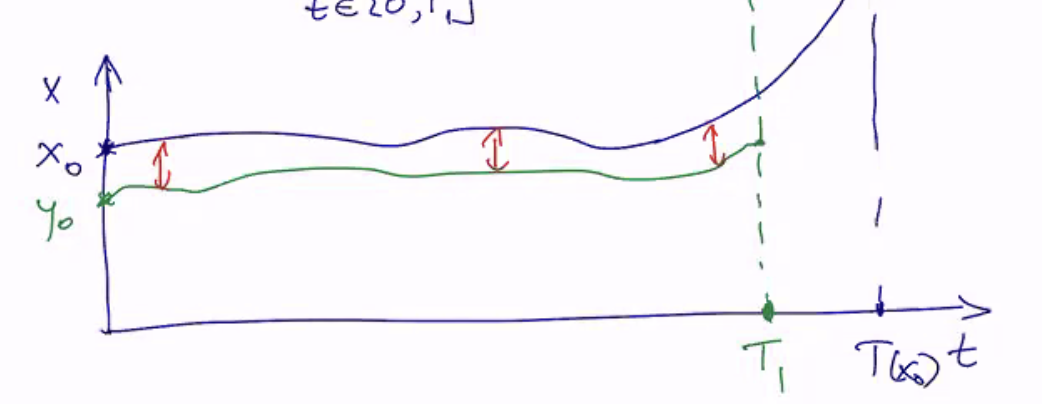
\includegraphics[scale=0.5]{localLipschitz.png}
\end{center}
\begin{thm}[Picard-Lindelof] Assume that $f$ is locally Lipschitz continuous.  Then the ODE is locally well-posed.
\end{thm}

\subsection{Contraction Principle}
We will use the "Contraction principle" - recall the following definitions:
\begin{definition}[Fixed-point Problem] Let $X$ be a Banach space,let $D \subset X$ be a closed subset of $X$, and let $F : D \rightarrow D$. Question: Can we solve the equation $F(u) = u$ where $u \in D$.
\end{definition}
\begin{definition}[Contraction] $$\|F(u) - F(v)\|_X \le L\|u - v\|,$$
where $L < 1$.
\end{definition}
If $F$ is a contraction, then it has a unique fixed point.  The existence proof follows an iterative construction: start with an arbitrary element $u_0 \in D$ and define $u_{n+1} = F(u_n)$.  We would show $\{u_n\}$ is a Cauchy sequence, so it converges.

We now prove the theorem.  We have $x' = f(x), x(0) = x_0$, so 
$$x(t) = x_0 + \int_{0}^t f(x(s))ds, t \in [0, T].$$
We choose $X = C[0, T; \R^n]$, $F(x)(t) = x_0 + \int_{0}^t f(x(s))ds.$ Then $x$ solves the ODE in $(0, T)$ if $F(x) = x$.
\begin{center}
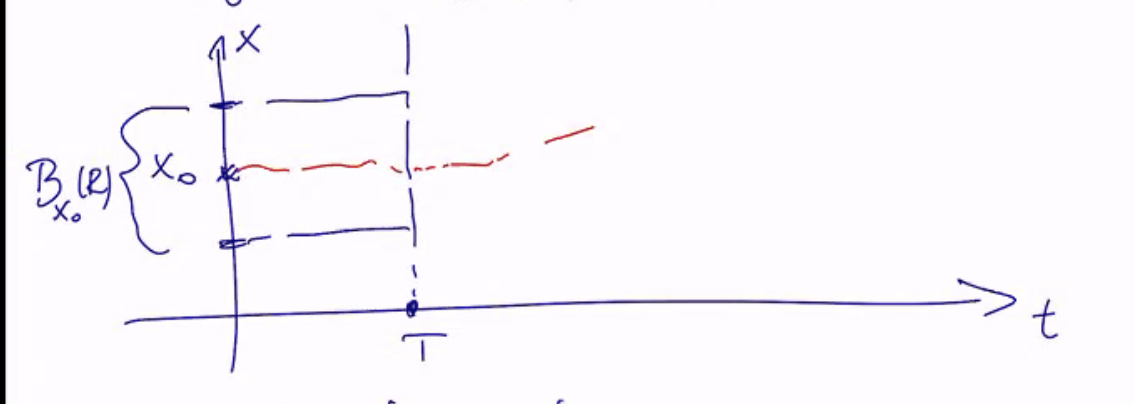
\includegraphics[scale=0.5]{ball.png}
\end{center}
We have to choose $R, T$.  Then
$$D = \{x \in X : \|x - x_0 \|_X \le R\}.$$

Let $R = |x_0|$.  Next, we choose $T$ so that $F : D \rightarrow D$ is Lipschitz.  For $F: D \rightarrow D$, we estimate the size of $F(x) - x_0$.
\begin{align*}
F(x)(t) - x_0| &= \left |\int_0^t f(x(s))ds\right | \\
&\le \left |\int_0^t f(x_0(s))ds\right | + \left | \int_0^t f(x) - f(x_0) ds \right | \\
&\le T |f(x_0)| + CT\|x - x_0\|_X  \\
\end{align*}
Hence,
$$\|F(x) - x_0\| \le T(|f(x_0)| + CR).$$
Thus, we choose $T$ such that $T(|f(x_0)| + CR) \le R$.

Now look at differences: For $x, y \in D$,
\begin{align*}
|F(x)(t) - F(y)(t)| &\le \int_{0}^t |f(x(s)) - f(y(s))| ds\\
&\le T C\sup_{s \in [0, T]} |x(s) - y(s)| \\
\end{align*}
thus,
$$\|F(x) - F(y)\|_X \le CT \|x - y\|_X,$$
so we can choose $T$ so that $CT\|x-y \|_X < 1$.

By the contraction principle, there exists a unique solution $x \in D$.  

To prove uniqueness of a solution, we have to show that any solution has to stay in $D$, up to time $T$.

\begin{center}
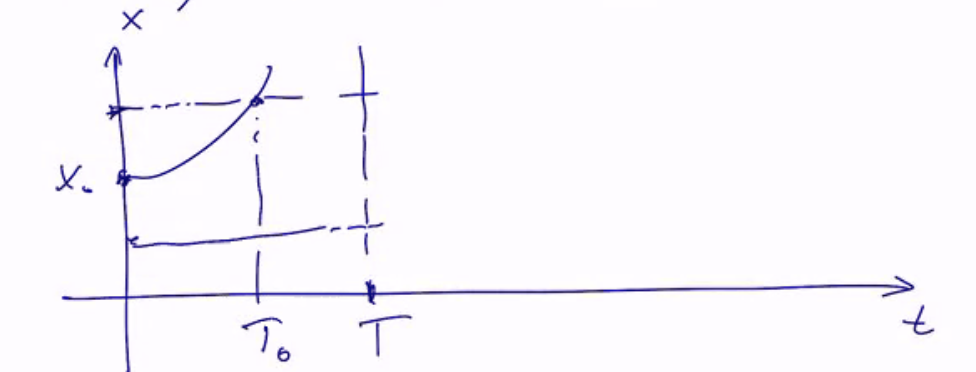
\includegraphics[scale=0.5]{unique.png}
\end{center}
Suppose a solution $\tilde{x}$ leave the ball before time $T$.  We repeat the above computation up to the exit time $T_0$.  Then, $T_0(|f(x_0) + CR|) < T$, since $T_0 < T$.  This is a contradiction since $T_0$ is the exit time.

\subsection{Bootstrap Argument}
Consider a bootstrap argument:  try to solve an equation and show that the solution $x$ satisfies some bound $\|x\|_T \le R$.  The difficulty is that a priori, we do not know any bound on $\|x\|_T$.  The solution:  make a bootstrap assumption, $\|x\|_T \le 2R$ and show that $\|x \|_T \le R$ under this assumption.  
\begin{center}
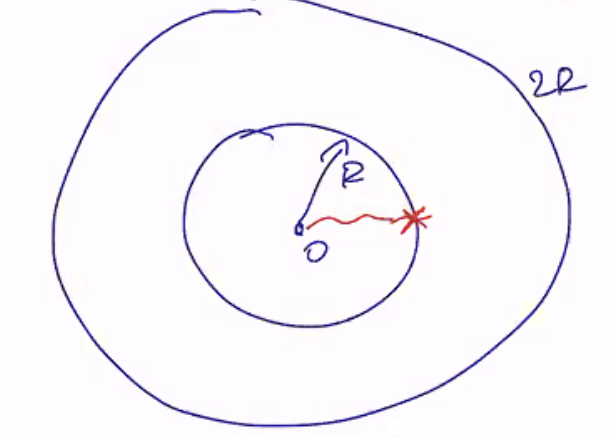
\includegraphics[scale=0.5]{bootstrap.png}
\end{center}

So far, we know uniqueness in $[0, T]$, where $T=T(x_0)$ given by the contraction argument.  We now show global uniqueness:  Suppose we have a solution $x_0$ with maximal lifespan $T_{max}(x_0)$.   Suppose $y$ is another solution.  We look at the maximal $T$ so that $x = y$ in $[0, T)$.  We now think of $T$ as the initial time.  We $x(T) = y(T)$ from continuity. Then, the solution is unique up to some time $T+T_0$, so $x = y$ in $[T, T+T_0]$, contradicting the maximality of $T$.  This is called a "continuity argument".

Next, we compare two solutions:  We have $x(0) = x_0, x: [0, T) \rightarrow R^n$.  We choose $T_1 < T$.  Then $x: [0, T_1] \rightarrow \R^n$.  We compare $x$ with a "nearby" solution $y(0) = y_0$ close to $x_0$.  We have$\|x\|_{X_{T_1}} \le R$ since we have continuity on a compact set.  We claim the following: if $|y_0 - x_0| < \epsilon$, then $x, y$ stay close.  We make a bootstrap assumption $\|y\|_{X_{T_1}} \le 2R$.  

$$\frac{d}{dt}|x-y|^2 = 2(x-y)(f(x) - f(y)) \le 2C|x-y|^2.$$

This is the \textit{Gronwall Inequality}.  It follows that $$|x-y|^2(t) \le e^{2ct}|x-y|^2(0) = e^{2ct}|x_0 - y_0|^2.$$
To close the bootstrap:
$$\|y\|_{X_{T_1}} \le \|x\|_{X_{T_1}} + \|x-y\|_{X_{T_1}} \le R + e^{cT_1}\|x_0 - y_0\| \le \frac{3R}{2},$$
which is better than the bootstrap assumption.
\section{September 8th, 2020}
Last lecture, we discussed the ordinary differential equation $x' = f(x)$ in $R^n$ with $x(0) = x_0$.  
We proved the Pircard-Lindelof theorem: if $f$ is locally Lip. then this problem is locally well-posed and the solution has a local Lip. dependence on the initial data.  We proved this by the contraction principle, using Picard iterations.
\subsection{Observations regarding Picard-Lindelof}
We note the following observations:
\begin{enumerate}
\item The result is local, so it can blow up in finite time.  

For example, take $x' = x^2, x(0) = x_0 > 0$.  The positive solutions to the ODE are $x(t) = \frac{1}{T - t}, T \ge 0$, where $T$ is the blow up time.  In this case, it is $T = \frac{1}{x_0}.$
\item If $f$ is not Lipschitz, then uniqueness might fail.

Take $x' = \sqrt{x}, x(0) = 0$.  An obvious solution is $x = 0$.  Other solutions are like $x(t) = ct^2$.  We can generate infinitely many solutions from here.
\begin{center}
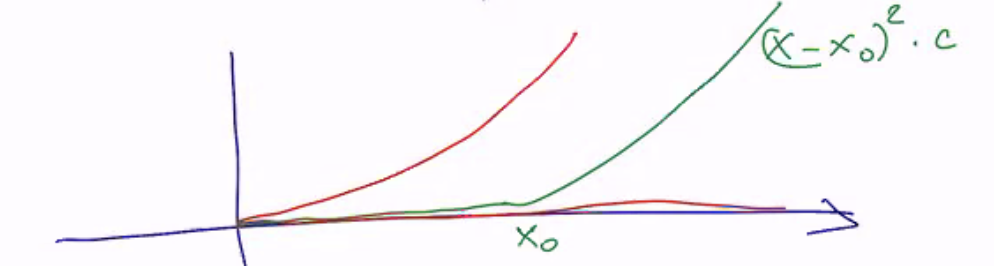
\includegraphics[scale=0.5]{notunique.png}
\end{center}
But solutions might still exist:
\begin{thm}[Peano] If $f$ is continuous, then a local solution exists.
\end{thm}
The proof uses Schauder's fixed point theorem.

\item What if $f \in C_{loc}^1$, the space of differentiable functions on a compact set?
\begin{thm} If $f \in C_{loc}^1$, then the flow map $x_0 \mapsto x(t, x_0) = \Phi(t, x_0)$ is of class $C^1$. 
\end{thm}
\begin{proof}
We give a sketch.  Take $x_0, x_0^h$ and assume $\frac{d}{dh}x_0^h(0)$ exists and show that $\frac{d}{dh}x^h$ exists.  The linearized equation about $h = 0$ is $\dot{y} = Df(x_0)y, y_0 = \frac{d}{dh}x_0^h$.  We expect that $$x^h(t) = x(t) + hy(t) + o(h).$$
Let $\tilde{x}^h(t) = x(t) + hy(t)$.  We claim that this is an "approximate solution", in the sense that $$\dot{\tilde{x}}^h(t) = f(\tilde{x}^h(t)) + o(h).$$
Furthermore, we have close initial data in the sense that
$$|x_0^h - \tilde{x}_0^h| \le o(h).$$
We repeat the difference bound for one exact and one approximate solution and show that 
$$|x^h(t) - \tilde{x}^h(t)| \le o(h)$$
\end{proof}
This implies that the Flow map is a group of local diffeomorphisms:
$$\Phi(t) \circ \Phi(s) = \Phi(t+s).$$
\end{enumerate}
\subsection{Linearization of an ODE}
The leads us to the notion of the linearization of the ODE: If we consider $x_0 \rightarrow x_0^h$, a one parameter family of data, assume this is $C^1$ in $h$.  The corresponding solution $x_0^h \rightarrow x^h(t)$ also in $C^1$ in $h$.  

What can we say about $$y^h(t) = \frac{d}{dh}x^h(t)?$$  We have $\dot{x}^h = f(x^h), x^h(0) = x_0.$  If we differentiate with respect to $h$, we have $\dot{y}^h = Df(x^h)y^h, y^h(0) = \frac{d}{dh}x_0^h.$, 
where $Df(x^h)$ is the differential of $f$, $\left (\frac{\partial f_i}{\partial x_j}\right )_{n\times m}$.   This is a linear ODE with variable coefficients.
\begin{center}
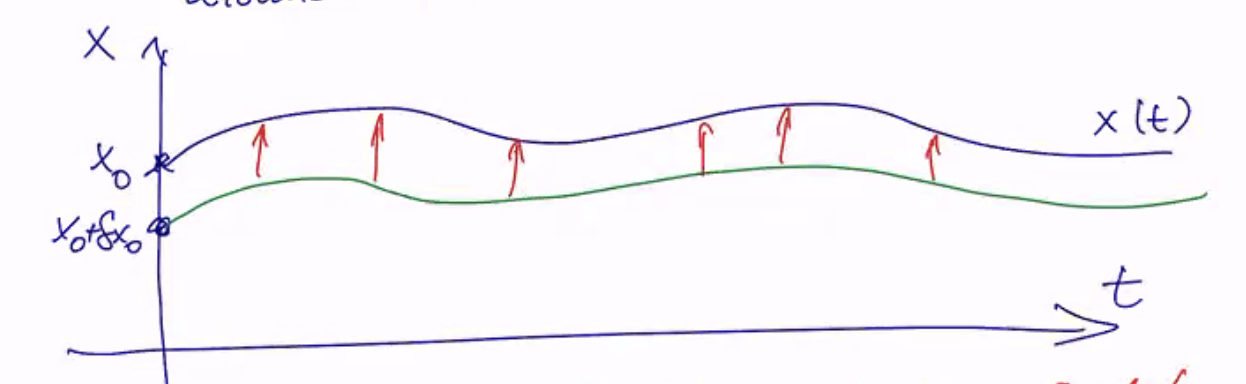
\includegraphics[scale=0.5]{linear.png}
\end{center}
\begin{proposition} If the linearized equation is well-posed, then we have Lip. dependence of solutions on the initial data.
\end{proposition}
\subsection{Our First Partial Differential Equation}
Our first example is scalar first order equations in $\R^n$, $$F(x, u, Du) = 0 \in \R^n, y:\R^n \rightarrow \R.$$
Today, we look at the case of linear, constant coefficients:
$$\sum a^i \partial_i u = f(x).$$
We will write this as $a^i \partial_i u$ following the Einstein summation convention.
Take $A = (a_1, \dots, a_n)$, so we have $A \cdot Du = f(x)$, with $A \ne 0$.  This can be interpreted as a directional derivative of $u$ in the direction $A$.
$$\frac{d}{dt}u(x(t)) = A \cdot Du(x(t)) = f(x(t)).$$
Note the fundamental theorem of calculus,
$$u(x(t)) = u(x_0) +\int_0^t f(x(t))dx.$$

Suppose we have a $C^1$ surface $\Sigma$ and we are asked to solve a $PDE$ with inidtial data $u = u_0$
 on $\Sigma$.  
 \begin{center}
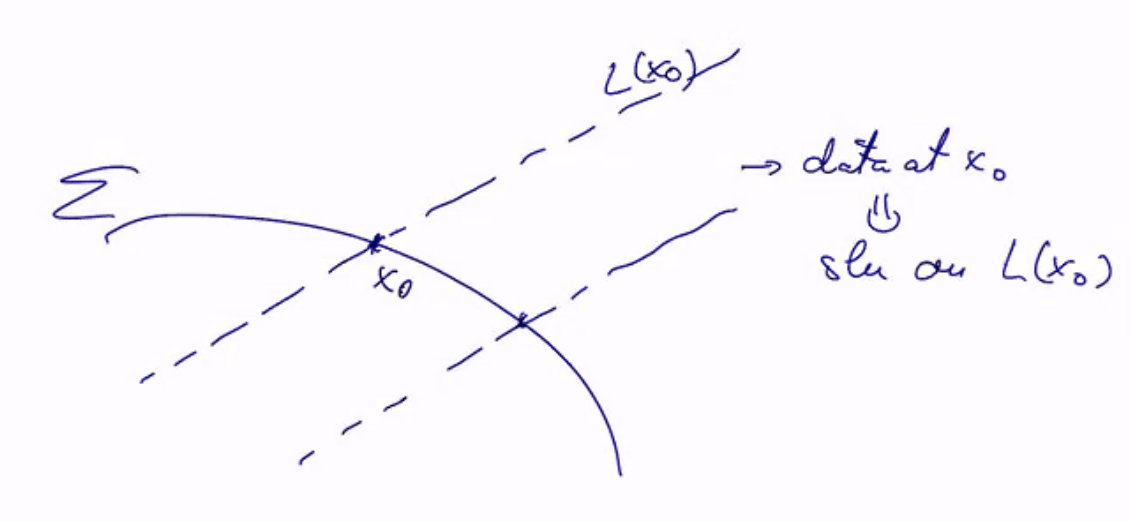
\includegraphics[scale=0.5]{sigma.png}
\end{center}
But things can go wrong.  If $\Sigma$ is a circle, we'd could have two intersection points.  Furthermore, we could miss the circle entirely and have no solutions.   Our solution in this case would be to assume that each line intersects $\Sigma$ exactly once.  However, if solutions are tangent, perturbations of the surface cause problems.  

To solve all these issues, we assume that $A$ is always transversal to $\Sigma$.  This can be written in terms of $N$, the normal vector to $\Sigma$, namely,
$$A \cdot N \ne 0.$$
\begin{definition}[Noncharacteristic Surface] If $A \cdot N \ne 0$, then we say the surface $\Sigma$ is noncharacteristic.
\end{definition}
 \begin{center}
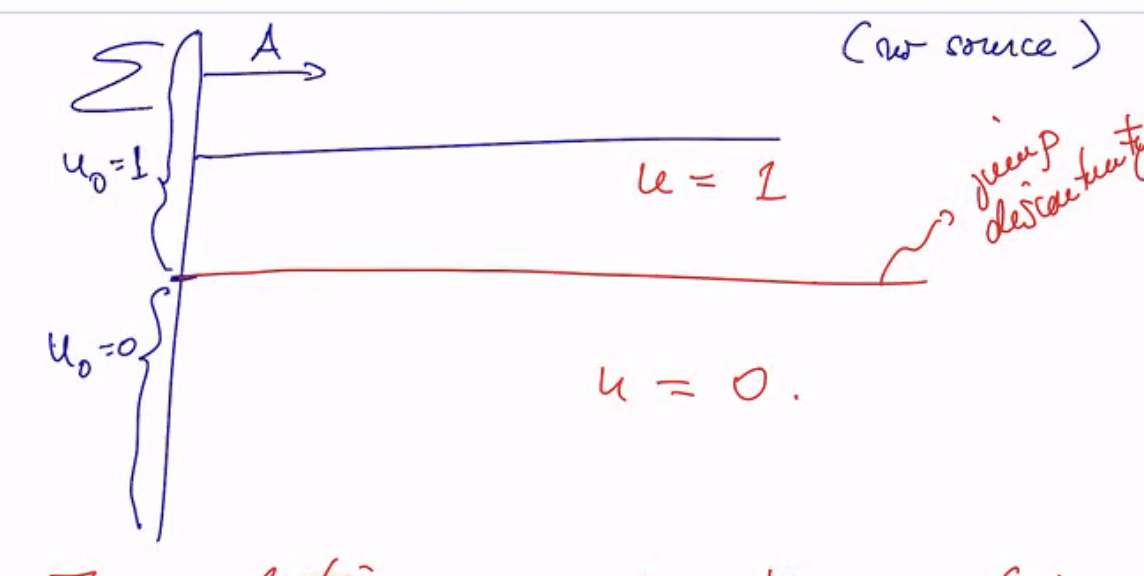
\includegraphics[scale=0.5]{bad.png}
\end{center}
We can have solutions that solve the equation at every point but not differentiable everywhere.
We learn 2 lessons from this example:
\begin{enumerate}
\item We need to enlarge the notion of what is a solution, this leads to the theory of distributions.
\item There are solutions to our PDE with a jump discontinuity along characteristic surfaces. ($\Gamma$ in the picture)
\end{enumerate}
After applying a change of coordinates, we have a Cauchy problem:
$$u_t + AD_x u = f, u(t=0) = u_0,$$
where $u_t$ is nonzero, corresponding to the condition that the surface is noncharacteristic.
\end{document}
